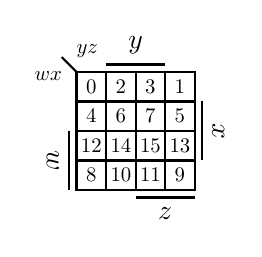
\begin{tikzpicture}[scale=0.75]
\def\sc{0.75};
\draw[thick] (0,0) -- ++(2,0) -- ++(0,2) -- ++(-2,0) -- cycle;
\draw[thick] (0,0.5) -- ++(2,0);
\draw[thick] (0,1) -- ++(2,0);
\draw[thick] (0,1.5) -- ++(2,0);
\draw[thick] (0.5,0) -- ++(0,2);
\draw[thick] (1,0) -- ++(0,2);
\draw[thick] (1.5,0) -- ++(0,2);
\draw[thick] (0,2) -- (-0.25,2.25);
\draw (-0.125,2.125) node[anchor=north east,scale=0.75]{$wx$};
\draw (-0.125,2.125) node[anchor=south west,scale=0.75]{$yz$};
\draw[thick] (-0.125,0) to node[sloped,below,rotate=180]{$w$} (-0.125,1);
\draw[thick] (2.125,0.5) to node[sloped,above,rotate=180]{$x$} (2.125,1.5);
\draw[thick] (0.5,2.125) to node[sloped,above]{$y$} (1.5,2.125);
\draw[thick] (1,-0.125) to node[sloped,below]{$z$} (2,-0.125);
\draw (0.25,1.75) node[scale=\sc]{0};
\draw (1.75,1.75) node[scale=\sc]{1};
\draw (0.75,1.75) node[scale=\sc]{2};
\draw (1.25,1.75) node[scale=\sc]{3};
\draw (0.25,1.25) node[scale=\sc]{4};
\draw (1.75,1.25) node[scale=\sc]{5};
\draw (0.75,1.25) node[scale=\sc]{6};
\draw (1.25,1.25) node[scale=\sc]{7};
\draw (0.25,0.25) node[scale=\sc]{8};
\draw (1.75,0.25) node[scale=\sc]{9};
\draw (0.75,0.25) node[scale=\sc]{10};
\draw (1.25,0.25) node[scale=\sc]{11};
\draw (0.25,0.75) node[scale=\sc]{12};
\draw (1.75,0.75) node[scale=\sc]{13};
\draw (0.75,0.75) node[scale=\sc]{14};
\draw (1.25,0.75) node[scale=\sc]{15};
\end{tikzpicture}